\section{Motivation}
\begin{frame}{Motivation: Why Do We Need RNNs?}
  \begin{figure}
    \centering
    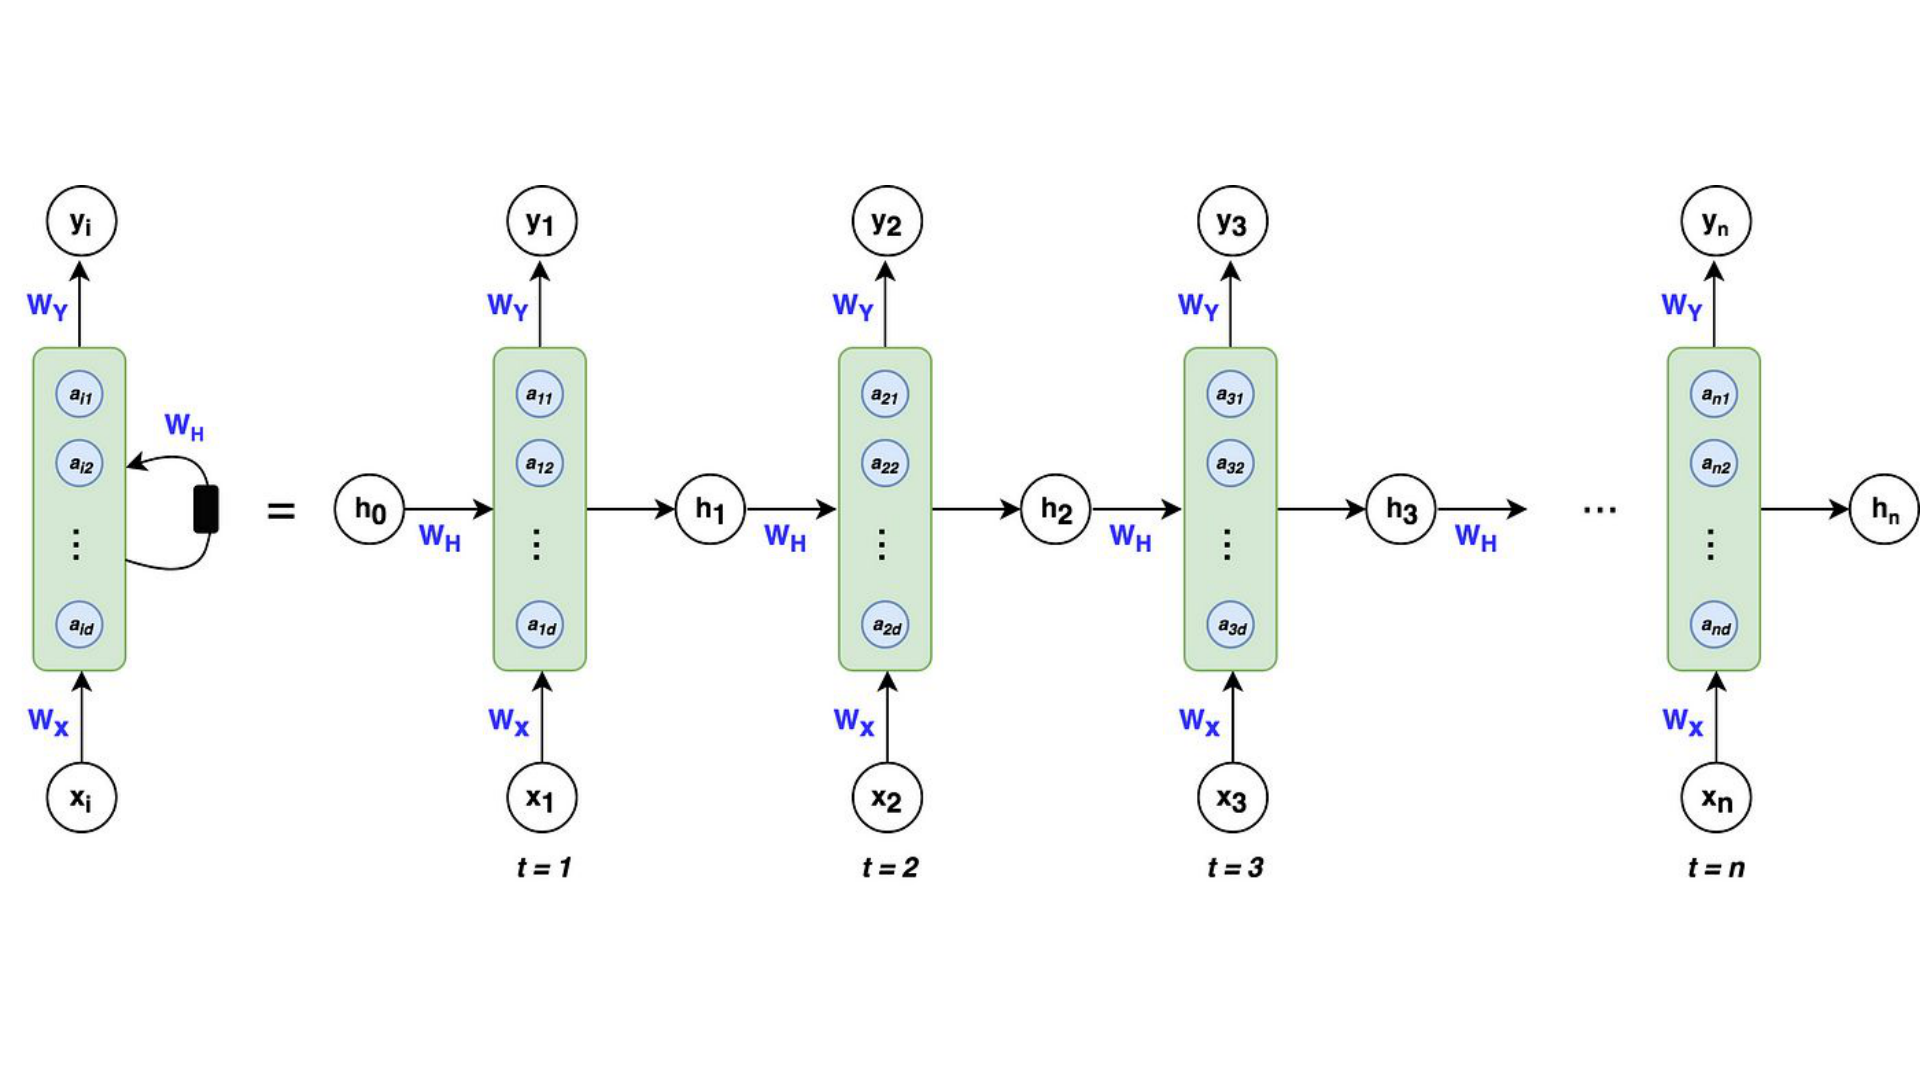
\includegraphics[width=0.9\paperwidth,height=0.7\paperheight,keepaspectratio]{images/rnn-lstm-gru/rnn_unrolled_computation_graph.png}
    \caption*{\tiny Source: B. Khuong, ``The Basics of Recurrent Neural Networks (RNNs),'' Towards AI, 2019}
  \end{figure}
\end{frame}

\begin{frame}{Motivation: Why Do We Need RNNs?}
\begin{itemize}
    \item Traditional feedforward networks don't handle sequential data effectively.
    \item Many applications (language modeling, time-series prediction, speech recognition) require memory of past inputs.
    \item RNNs enable temporal dynamic behavior by maintaining hidden states.
\end{itemize}
\textbf{Examples Where Order Matters:} 
\begin{itemize}
    \item Translating ``I am happy'' vs ``Happy I am''
    \item Predicting next stock price based on past trends 
    \item Understanding a sentence word-by-word 
\end{itemize}
\textbf{Key Idea:} Add a feedback loop to remember previous computations.
\end{frame}